\chapter{Description of the effect of perturbative fields on arcs}
Put the motivation
\section{Pseudo-Elliptical Models}
The Pseudo-Elliptical models come from the distortion of the lensing potential, in which
the radial coordinate $r$ is replaced by $\xi$, i.e $\phi(r)\rightarrow \phi(\xi)$, where
\bea
\xi &=&r_0\,x_\eta=r_0\sqrt{x^2_{1\eta}+x^2_{2\eta}} \label{pe_cord} \\
x_{1\eta}&=&\sqrt{\ae} x_1\\
x_{2\eta}&=&\sqrt{\be} x_2
\eea
where $r_0$ is a scaling parameter (model dependent), $\ae$ and $\be$ are the parameter
defining the ellipticity.

The most common parameterizations for the ellipticity are

\begin{eqnarray}
\ae=1-\eta &\qquad& \be =1+\eta \label{par_gk}\\
\ae=1-\eta &\qquad & \be =\dfrac{1}{1-\eta} \label{par_gen}
\end{eqnarray}
where the Eq.~ (\ref{par_gk}) corresponds to the parametrization of the
Angle Deflection Model ($\eta=\varepsilon$ following the notation of  Golse \& Kneib 2002)
and the other one, Eq.~ (\ref{par_gen}),  corresponds to the standard parametrization ($\eta=\varepsilon_\varphi$
following the notation of Meneghetti et al 2002).

Working in polar coordinates $x_1=x\cos{\te}$ + $x_2=x\sin{\te}$ we get to

\beq
\xi=r\sqrt{\ae \cos^2{\te}+\bf \sin^2{\te}}.
\label{pe_radius}
\eeq

Regarding the Perturbative Approach, we can write any Pseudo-Elliptical Model as

\beq
\phi_{_\mathrm{PE}}(r)=\phi_0(r)+\phi(\xi)-\phi_0(r), \quad \psi_{_\mathrm{PE}}(r)=\phi(\xi)-\phi_0(r).
\label{pe_model}
\eeq

Here, we use the following notation

\begin{eqnarray*}
\phi_\xi\equiv \phi(\xi), &\quad&  \phi^\prime_\xi \equiv \dfrac{d\phi(\xi)}{d\xi}, \quad \phi^{\prime\prime}_\xi \equiv \dfrac{d^2\phi(\xi)}{d\xi^2}\\
\phi_0\equiv \phi(r),&\quad&  \phi^\prime_0 \equiv \dfrac{d\phi(r)}{dr}\\
\xer \equiv \re \sqrt{\ae \cos^2{\te}+\be\sin^2{\te}},&\quad& \scriptg(\eta,\te)=\re^2\mathcal{A}(\eta)\sin{(2\te)},\quad \mathcal{A}(\eta)=\be-\ae
\end{eqnarray*}

The, we will begin to derive the analytical expression for the main fields of the Perturbative Method. Using the 
definition, we have

\beq
f_0(\te)=\phi(\xer)-\phi_0(\re)
\eeq
then, its derivative respect to $\te$ is
\beq
\frac{df_0}{d\te}=\dfrac{d\phi_{\xer}}{d\xer}\dfrac{d\xer}{d\te}=\frac{1}{2}\dfrac{\phi^\prime_{\xer}}{\xer}\scriptg(\eta,\te)
\label{df0_pe}
\eeq
where, we used 
\beq
\dfrac{d\xer}{d\te}=\frac{1}{2}\dfrac{\scriptg(\eta,\te)}{\xer}.                 
\label{dxer_pe}
\eeq

From Eqs.{(\ref{pe_radius}, \ref{pe_model})} is easily get to

\begin{equation*}
\dfrac{\prtl \psi_{_{\mathrm{PE}}}(r) }{\prtl r}=\dfrac{d\phi_\xi}{d\xi}\dfrac{\prtl \xi}{\prtl r}-\dfrac{\prtl \phi_0}{\prtl r}
\end{equation*}

Evaluating at the Einstein Radius, we have
\beq
f_1(\te)=\dfrac{\xer}{\re}\phi^\prime_{\xer}-\phi^\prime_0
\label{f1_pe}
\eeq

Also, making the derivative of Eq.~(\ref{df0_pe}) respect to $\te$, is straightforward get to
\beq
\dfrac{d^2f_0}{d\te^2}=\frac{1}{2}\scriptg_\te(\eta,\te)\dfrac{\phi^\prime_{\xer}}{\xer}+%
\frac{1}{4}\left[ \dfrac{\scriptg(\eta,\te)}{\xer}\right]^2\left(\phi^{\prime\prime}_{\xer}-\dfrac{\phi^{\prime}_{\xer}}{\xer}  \right)
\label{ddf0_pe}
\eeq
where $\scriptg_\te(\eta,\te)\equiv d\scriptg(\eta,\te)/d\te$.

Now, to write the expression of $d^nf_0/d\te$ and $f_1$ as function of the lensing functions, we use some basic relationships valid for
any circular model

\bea
\phi^\prime &\equiv& \dfrac{d\phi(r)}{d r}=\alpha(r) \label{dphi}\\
\phi^{\prime\prime}&\equiv& \dfrac{d^2\phi(r)}{d r^2}=2\kappa(r)-\dfrac{\alpha(r)}{r}\label{ddphi}\\
\gamma(r)&=&\dfrac{\alpha(r)}{r}-\kappa(r)
\eea

Then, using these relationships and as $r$ is a dummy variable, we have for the main fields
\bea
\dfrac{df_0}{d\te}&=& \frac{1}{2}\dfrac{\alpha(\xer)}{\xer}\scriptg(\eta,\te) \label{df0_pe2}\\
f_1(\te)&=&\dfrac{\xer}{\re}\alpha(\xer)-\alpha(\re) \label{f1_pe2}
\eea
and also, we have
\beq
\label{ddf0_pe2}
\dfrac{d^2f_0}{d\te^2}=\frac{1}{2}\scriptg_\te(\eta,\te)\dfrac{\alpha(\xer)}{\xer}-%
\frac{\gamma(\xer)}{2}\left[ \dfrac{\scriptg(\eta,\te)}{\xer}\right]^2 
\eeq

\subsection{Expression for small values of the ellipticity}

Now, we will expand the analytical expressions for the main fields 
Eqs.(\ref{df0_pe2}, \ref{f1_pe2}) in Taylor Series around $\eta=0$. 
Is straightforward verify that

\bea
\dfrac{df_0}{d\te}& \approx & \eta\alpha(\re)\re\sin{(2\te)} \label{df0_pe_appr}\\
f_1(\te)&\approx&-\eta \kappa(\re)\re\cos{(2\te)} \label{f1_pe_appr}
\eea

And from the  Eq.~(\ref{df0_pe_appr}), or making the Taylor Series in the Eq.~(\ref{ddf0_pe2}), we get
to
\beq
\dfrac{d^2f_0}{d\te^2}=2\eta\alpha(\re)\re\cos{(2\te)} \label{ddf0_pe_appr}
\eeq

For example, if we considerer and Pseudo-Elliptical SIS (setting $\re=1$) we get to the
Eqs.(17) of Alard's Paper 2008 (without considering the contribution of substructures), i.e,
\begin{eqnarray*}
 f_1(\te)&\approx&-\frac{\eta}{2}\cos{(2\te)}\\
 \dfrac{df_0}{d\te}& \approx & \eta\sin{(2\te)} 
\end{eqnarray*}
 


\pagebreak

\section{Elliptical Models (Gabriel)}

\section{Substructures}
\begin{wrapfigure}{r}{0.4\textwidth}
  \begin{center}
%  \centering{\epsfig{Fig_subsstructure.eps,width=0.45\textwidth}}
   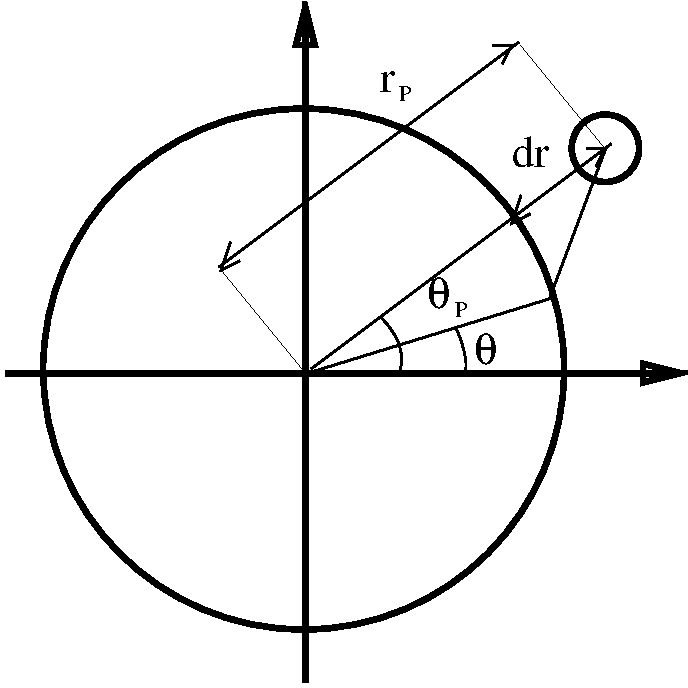
\includegraphics[width=0.30\textwidth]{graphics/Fig_subsstructure.pdf}
  \end{center}
    \caption{Geometry of the perturbation induced by the substructure. The great circle corresponds to Einstein Ring,
  while the small one represent the substructure located at $r_p=\re +\zeta$.}
\end{wrapfigure}

We can considerer the perturbation as
\begin{equation}
\psi_{ss}(r,\te,\pi_p)=\varphi(\zeta)
\end{equation}
where $\varphi$ corresponds to a central potential (circular model, like SIS, NFW and so on) and $\pi_p$
are the substructure parameters, like mass, position and inclination. $\zeta$ comes from the Fig. 1 ($dr=\zeta$)
where
\begin{eqnarray}
\vec{r}_p&=&r_p\cos{\tep}\hat{\imath} + r_p\sin{\tep}\hat{\jmath}\\
\vec{r}&=&r\cos{\te}\hat{\imath} + r\sin{\te}\hat{\jmath}\\
\vec{\zeta}&=&\vec{r}_p-\vec{r}.
\end{eqnarray}
Taking the modulus of $\zeta$, is straightforward to verify that
\begin{equation}
\zeta(r,\te)=\sqrt{r^2-2r r_p\cos{(\te-\tep)}+r^2_p}.
\label{xirte}
\end{equation}

Before give the analytical expression for the fields $f_1$ and $d^nf_0/d\te^n$ ($n=1,2$), we will
give some useful results (with $\zeta\equiv\zeta(r,\te)$).
\begin{eqnarray}
\dfrac{d\zeta}{d\te}&=&\dfrac{r r_p \sin{(\te-\te_p)}}{\zeta}=\dfrac{\Omega(\zeta)}{\zeta}=\\
\dfrac{d\Omega(\zeta)}{d\te}&=&r r_p\cos{(\te-\te_p)}\\
\dfrac{d\zeta}{dr}&=&\dfrac{r-r_p\cos{(\te-\te_p)}}{\zeta}
\end{eqnarray}

Introducing the following notation $\varphi_\zeta\equiv \varphi(\zeta) $, $\varphi^\prime_\zeta=d\varphi_\zeta/d\zeta$, $\varphi^{\prime\prime}_\zeta=d^2\varphi_\zeta/d\zeta^2$
and using the relations above we have.

\begin{eqnarray}
\dfrac{\prtl \psi_{ss}}{\prtl \te}&=&\Omega(\zeta)\dfrac{\varphi^\prime}{\zeta}\label{df0}\\
\dfrac{\prtl^2 \psi_{ss}}{\prtl\te^2}&=&\left[\varphi^{\prime\prime}_\zeta-\dfrac{\varphi^\prime_\zeta}{\zeta}\right]%
\left(\dfrac{\Omega(\zeta)}{\zeta}\right)^2+[r r_p\cos{(\te-\tep)}]\dfrac{\varphi^\prime_\zeta}{\zeta}\label{ddf0}\\
\dfrac{\prtl \psi_{ss}}{\prtl r}&=&[r-r_p\cos{(\te-\tep)}]\dfrac{\varphi^\prime_\zeta}{\zeta}\label{f1}
\end{eqnarray}

Using the Eqs.~(\ref{dphi},\ref{ddphi}) and as $r$ is dummy variable, we can define $\al_\zeta=\al(\zeta)=\varphi^\prime_\zeta$ and $\kappa_\zeta=\kappa(\zeta)$. From the
Eqs.(\ref{xirte}, \ref{df0}-\ref{f1}) (evaluated at $r=\re$), we get to the analytical expression for the main fields of
the perturbative approach as function of the angle deflection and convergence, i.e.
\begin{eqnarray}
\dfrac{df_0}{d\te}&=&\al_{\xie}\dfrac{\Omega(\xie)}{\xie}\\
\dfrac{d^2f_0}{d\te^2}&=&2\left[\kappa_{\xie}-\dfrac{\al_{\xie}}{\xie}\right]%
\left(\dfrac{\Omega(\xie)}{\xie}\right)^2+\al_{\xie}\dfrac{[\re r_p\cos{(\te-\tep)}]}{\xie}\\
f_1&=&\al_{\xie}\dfrac{[\re-r_p\cos{(\te-\tep)}]}{\xie},
\end{eqnarray}

\subsection{SIS model as substructure}

As application of these analytical expression, we will considerer the case of the Singular Isothermal Sphere, for
which $\psi(r,\te,\pi_p)=m_p\zeta$, where $m_p$ is the mass contained at the critical radius.
Is very easy to verify that $\al_\zeta=m_p$,  $\kappa_\zeta=m_p/(2\zeta)$ (this expression comes from the usual
definition of the SIS convergence) and therefore we get to
\begin{eqnarray}
\dfrac{d f_0}{d\te}&=&\dfrac{\re m_p r_p \sin{(\te -\tep)}}{\sqrt{\re^2-2\re r_p\cos{(\te-\tep)}+r^2_p}}.\\
f_1&=&\dfrac{m_p[\re-r_p\cos{(\te-\tep)}]}{\sqrt{\re^2-2\re r_p\cos{(\te-\tep)}+r^2_p}}.
\end{eqnarray}
If we choose $\re=1$ we get to the expression given in Alard's Paper 2008.

Besides, the another quantity useful to calculate the critical and caustic lines is
\begin{equation}
\dfrac{d^2 f_0}{d\te^2}=\dfrac{m_p}{\sqrt{\re^2-2\re r_p\cos{(\te-\tep)}+r^2_p}}%
\left[\re r_p\cos{(\te-\tep)}- \dfrac{[\re r_p\sin{(\te-\tep)}]^2}{\re^2-2\re r_p\cos{(\te-\tep)}+r^2_p} \right].
\end{equation}

Conclusions: Now, we are able to considerer another kind of substructure that come from circular lenses.


\section{External Shear + Continuous Matter}

Objects near the main lens galaxy or along the line of sight often perturb the lensing potential.
In the case that we are considering the contribution of the mass distribution external to the lens,
we can work with the potential coming from the external mass + external shear.
\beq
\phi(r)=\phi_0(r)+\frac{r^2}{2}\left[ \kex-\gex\cos{2(\te-\te_\gamma)}\right].
\eeq
where the perturbative potential, in this case is
\beq
\psi_{_{\mathrm{EX}}}(r)=\frac{r^2}{2}\left[ \kappa_{_{\mathrm{EX}}}-\gamma_{_{\mathrm{EX}}}\cos{2(\te-\te_\gamma)}\right]
\eeq
From the expression above, is easy get to
\bea
f_1(\te)&=& \re\left[\kex-\gex\cos{2(\te-\te_\gamma)}   \right]\\
\dfrac{d f_0}{d\te} (\te)&=& \re^2\gex\sin{2(\te-\te_\gamma)}\\
\dfrac{d f^2_0}{d\te^2}(\te)&=& 2\re^2\gex\cos{2(\te-\te_\gamma)}\\
\eea

Note that this model for perturbation is the most simples, but don't forget that $\re$ depends on the
unperturbed potential, for example: could be NFW, SIS, Cuspy-NFW, etc etc. 